\chapter{ManagedIrbis. Быстрый старт}

У попа была собака. Он её любил. Она съела кусок мяса. Он её убил. В землю закопал. Надпись написал. У попа была собака. Он её любил. Она съела кусок мяса. Он её убил. В землю закопал. Надпись написал.

У попа была собака. Он её любил. Она съела кусок мяса. Он её убил. В землю закопал. Надпись написал. У попа была собака. Он её любил. Она съела кусок мяса. Он её убил. В землю закопал. Надпись написал. У попа была собака. Он её любил. Она съела кусок мяса. Он её убил. В землю закопал. Надпись написал.

У попа была собака. Он её любил. Она съела кусок мяса. Он её убил. В землю закопал. Надпись написал.

У попа была собака. Он её любил. Она съела кусок мяса. Он её убил. В землю закопал. Надпись написал.

У попа была собака. Он её любил. Она съела кусок мяса. Он её убил. В землю закопал. Надпись написал. У попа была собака. Он её любил. Она съела кусок мяса. Он её убил. В землю закопал. Надпись написал.

\begin{figure}[h]
	\centering
	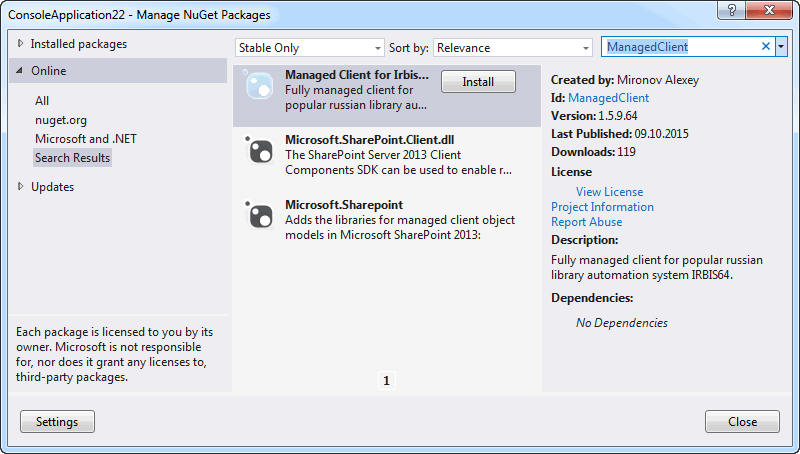
\includegraphics[width=0.7\textwidth]{nuget}
	\caption{Подключение библиотеки через NuGet}
\end{figure}


\begin{lstlisting}
using System;
using System.Linq;

using ManagedIrbis;

class Program
{
  private static void Main()
  {
    try
    {
      using (ManagedIrbis client = new ManagedIrbis())
      {
        // Подключаемся к серверу
        client.ParseConnectionString("host=127.0.0.1;port=6666;"
                                     + "user=1;password=1;");
        client.Connect();

        // Ищем все книги, у которых автор начинается на А (кириллица)
        int[] foundRecords = client.Search("\"A={0}$\"", "А");

        // Чтобы не распечатывать все найденные записи,
        // ограничимся первыми 10
        int recordsToShow = Math.Min(foundRecords.Length, 10);

        for (int i = 0; i < recordsToShow; i++)
        {
          int thisMfn = foundRecords[i];

          // Считываем запись
          MarcRecord record = client.ReadRecord(thisMfn);

          // Получаем основное заглавие
          string mainTitle = record
            .Fields
            .GetField("200")
            .GetSubField('a')
            .GetSubFieldText()
            .FirstOrDefault();

          // Можно было просто написать: 
          // string mainTitle = record.FM("200", 'a');

          Console.WriteLine
            (
              "MFN={0}, Main title={1}",
              thisMfn,
              mainTitle
            );

          // Расформатируем запись
          Console.WriteLine
            (
              "BRIEF: {0}",
              client.FormatRecord("@brief", record)
            );

          // Создаем запись
          MarcRecord newRecord = new MarcRecord();
          newRecord.AddField
            (
              "700",
              'a',
              "Управляемый клиент ИРБИС64"
            )
            .AddField
            (
              "200",
              'a', 
              string.Format ("Новая Запись от {0}", DateTime.Now),
              'f',
              "Управляемый клиент"
            );

          // Отсылаем вновь созданную запись на сервер
          client.WriteRecord
            (
              newRecord, 
              false, 
              true
            );

          Console.WriteLine(new string('-', 60));
        }

        // По выходу из using автоматически вызывается client.Disconnect ()
      }
    }
    catch (Exception ex)
    {
      Console.WriteLine(ex);
    }
  }
}\end{lstlisting}
